% figure: 线代-正交投影.png
% 用途：线代 03-2 向量的内积与正交 —— 正交投影 p=(b,a)/(a,a)·a 与残差 b−p⊥a
%       （同一张图也用于 2007 数二第 24 题：把向量沿特征方向分解，拼出 B=(E−P)−2P）
% 构建：..\build.ps1 -File .\vec-orthogonal-projection.tex
% 说明：直线取水平、残差取竖直，"垂直"一眼可见；全部标签都离开线（b 在箭头上方、
%       p 在直线下方、b−p 在残差右侧），并加白底遮罩，不压线。
\documentclass[border=10pt]{standalone}
\usepackage{fontspec}
\setmainfont{Cambria}
\usepackage{unicode-math}
\setmathfont{Cambria Math}
\usepackage{tikz}
\usetikzlibrary{calc}
\usepackage{ctex}

\definecolor{figink}{HTML}{1E2228}      % 图线主色（投影向量与残差）
\definecolor{figacc}{HTML}{B23020}      % 强调色（原向量 b）
\definecolor{figsub}{HTML}{606874}      % 次要（直线 L 与说明文字）

\begin{document}
\begin{tikzpicture}[x=1cm, y=1cm, line width=1.1pt, line cap=round, line join=round]
  \coordinate (O) at (0,0);
  \coordinate (P) at (4.6,0);       % 垂足：b 的终点在 L 上的投影
  \coordinate (B) at (4.6,3.1);     % 向量 b 的终点

  % 直线 L（虚线，两端留余量）
  \draw[figsub, line width=0.5pt, dashed] (-0.5,0) -- (6.9,0);

  % 向量 b、投影 p、残差 b−p
  \draw[figacc, ->, line width=1.6pt] (O) -- (B);
  \draw[figink, ->, line width=1.6pt] (O) -- (P);
  \draw[figink, dashed, line width=1.1pt] (P) -- (B);

  % 垂足处的直角标记（向左上）
  \draw[figink, line width=1.0pt]
    ($(P)+(-0.42,0)$) -- ($(P)+(-0.42,0.42)$) -- ($(P)+(0,0.42)$);

  % 端点
  \fill[figink] (O) circle (1.5pt);
  \fill[figacc] (B) circle (1.9pt);

  % 标签：全部离开线，白底遮罩
  \node[figacc, fill=white, inner sep=1.5pt] at (1.9,1.80) {$b$};
  \node[figink, fill=white, inner sep=1.5pt] at (2.7,-0.52) {$p$};
  \node[figink, fill=white, inner sep=1.5pt, anchor=west] at (4.95,1.60) {$b-p$};
  \node[figsub, fill=white, inner sep=1.5pt, anchor=west] at (5.80,0.30) {$L$};
  \node[figsub, fill=white, inner sep=1.5pt, anchor=east] at (-0.30,-0.40) {$O$};

  % 图下说明（两行，贴图放，避免整体过高）
  \node[anchor=west, align=left] at (-0.5,-1.55)
    {$p=\dfrac{(b,a)}{(a,a)}\,a$：$p$ 沿 $a$ 方向，是 $b$ 在直线 $L$ 上的“影子”};
  \node[figsub, anchor=west, align=left] at (-0.5,-2.35)
    {$b=p+(b-p)$，且 $(b-p)\perp a$——影子加残差正好还原 $b$};
\end{tikzpicture}
\end{document}
